%%% Local Variables:
%%% mode: latex
%%% TeX-master: "../index"
%%% End:

% Recommended:
% Complexity of collisions (preimage)
% - Birthday paradox
% How to build hash functions
% - Blocks with padding
% - Merkle-Damgaard
% - Why is it secure?

\subsection*{Agenda}
\begin{enumerate}
\item Birthday paradox
\item Complexity of collisions
\item Iterated hash functions
\item Padding
\item Merkle-Damgård
\end{enumerate}
\subsection{Properties of Hash functions}

\textbf{Hash functions} takes a input of a binary string of arbitrary
length and returns a binary string of fixed length.
\begin{figure}[H]
  \begin{centering}
    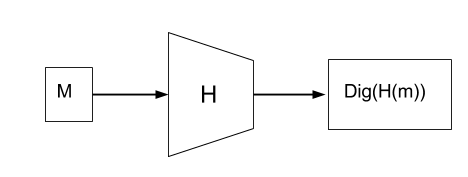
\includegraphics[scale=0.4]{images/10-hash}
    \caption{Model for hashing a message}
  \end{centering}
\end{figure}

\textbf{The ideal Hash function} has 4 main properties:
\begin{itemize}
\item [--]it is easy to compute the hash value for any given message
\item [--]it is infeasible to generate a message that has a given hash
\item [--]it is infeasible to modify a message without changing the hash
\item [--]it is infeasible to find two different messages with the same hash.
\end{itemize}

\textbf{Security of Hash functions} 

% \textbf{Private key:}

% \textbf{Private key:}

\subsection{Birthday paradox}



\subsection{Iterated Hash functions}

\subsection{Padding}
\begin{figure}[H]
  \begin{centering}
    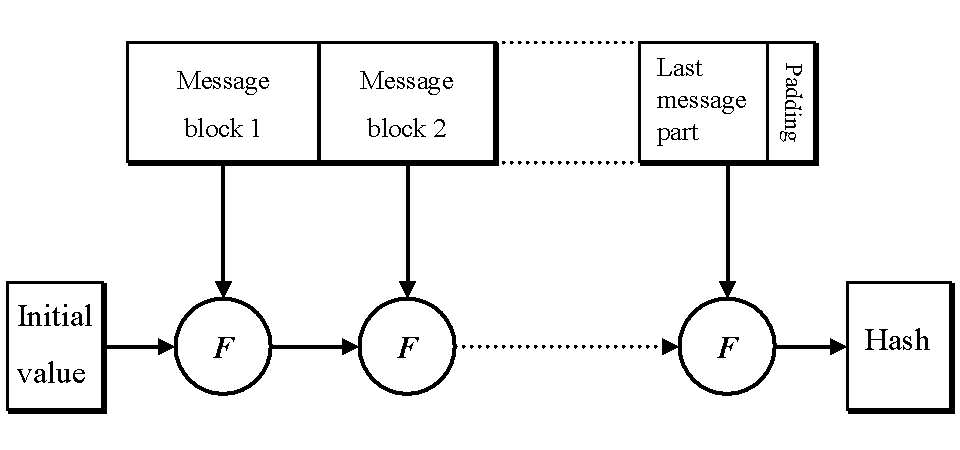
\includegraphics[scale=0.3]{images/10-padding}
    \caption{Model for hashing using padding}
  \end{centering}
\end{figure}
\subsection{Merkel-Damgård}

